\documentclass[acmtog]{acmart}
\usepackage{graphicx}
\usepackage{subfigure}
\usepackage{natbib}
\usepackage{listings}
\usepackage{bm}
\usepackage{float}
\definecolor{blve}{rgb}{0.3372549 , 0.61176471, 0.83921569}
\definecolor{gr33n}{rgb}{0.29019608, 0.7372549, 0.64705882}
\makeatletter
\lst@InstallKeywords k{class}{classstyle}\slshape{classstyle}{}ld
\makeatother
\lstset{language=C++,
	basicstyle=\ttfamily,
	keywordstyle=\color{blve}\ttfamily,
	stringstyle=\color{red}\ttfamily,
	commentstyle=\color{magenta}\ttfamily,
	morecomment=[l][\color{magenta}]{\#},
	classstyle = \bfseries\color{gr33n},
	tabsize=2
}
\lstset{basicstyle=\ttfamily}

% Title portion
\title{Assignment 2:\\ {}}

\author{Name:\quad Zhang Siyuan  \\ student number:\ 2019533240
\\email:\quad zhangsy3@shanghaitech.edu.cn}

% Document starts
\begin{document}
\maketitle

\vspace*{2 ex}

\section{Introduction}
	This assignment implements:
\begin{itemize}
	\item [1)] the basic iterative de Casteljau Bézier vertex evaluation algorithm.
	\item [2)] constructing Bézier surfaces with the normal evaluation at each mesh vertex.
	\item [3)] rendering the Bézier surfaces based on the vertex array.
	\item [4)] creating more complex meshes by stitching multiple Bézier surface patches together.
	\item [5)] constructing the B-Spline surfaces.
	\item [6)] the adaptive mesh construction based on the curvature estimation.
	\item [7)] calculating the curvature on each vertex.
\end{itemize}

\section{Implementation Details}
\subsection{de Casteljau Bézier Algorithm and Normal}
\begin{figure}[h]
	\centering
	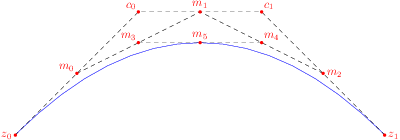
\includegraphics[height = 2.4cm]{bezier_curve_example.png}
	\caption{example for drawing a bezier curve}
\end{figure}

A Bézier curve $B$ (of degree $n$,
with control points $\beta_{0},\ldots ,\beta_{n}$)
can be written in Bernstein form as follows
$$
	B(t)=\sum _{i=0}^{n}\beta_{i}b_{i,n}(t)
$$
where $b$ is a Bernstein basis polynomial
$$
	b_{i,n}(t)={n \choose i}(1-t)^{n-i}t^{i}
$$
\subsubsection{Simple Implication}
So we can imply the algorithm with a double loop over the control points:
\begin{lstlisting}[language=C++]
position de_casteljau(t, ControlPoints):
    beta = ControlPoints;
    n = beta.size;
    for j = (0..n-1):
        for k = (0..n - j - 1):
            beta[k] = beta[k] * (1 - t) +
				      beta[k + 1] * t;
    return beta[0];
\end{lstlisting}
\\
\subsubsection{How about Normal}
So as to get the normal of each vertex,
we must get the tangent of the vertex on both the x, y direction.
Seeing that on a curve, the tangent of the vertex is the direction of the last
iterated two vertices.
A recursive function to get the tangent and the position as follows:
\begin{lstlisting}[language=C++]
vertex evaluate(control_points, t):
    if (control_points.size() == 2)
    	x.position = (1 - t) * control_points[0] +
		             t * control_points[1];
        x.tangent = control_points[1] -
		            control_points[0];
        return x;
    else:
        vector<position> next_control_points;
        first_vertex = control_points[0];
        for i = (1..control_points.size() - 1):
            second_vertex = control_points[i];
            next_control_points.push_back(
				(1 - t) * first_vertex +
			          t * second_vertex);
            first_vertex = second_vertex;
        return evaluate(next_control_points, t);
\end{lstlisting}
\\
So the normal of the vertex can be calculated as follows:
\begin{lstlisting}[language=C++]
normal = normalize(cross(
	evaluate(control_points_on_x_direction, u).tangent,
	evaluate(control_points_on_y_direction, v).tangent));
\end{lstlisting}
\subsection{$K^{th}$ Order Derivatives and Curvature}
\subsubsection{$K^{th}$ Order Derivatives}
The $K^{th}$ order derivative of a Bessel curve as follows:
$$
C^{(k)}(t) = n(n-1)\dots(n-k+1)\sum_{i=0}^{n-k}B_{i,n-k}p_{i}^{(k)}
$$
$$
p_{i}^{(k)} = p_{i+1}^{(k-1)} - p_{i}^{(k-1)}
$$
So we can calculated any derivative of any order as follows:
\begin{lstlisting}[language=C++]
vec3 at(control_points, t, derivative_order):
    beta = control_points;
    n = beta.size;
    prefix = 1;
    for i = (0..derivative_order - 1):
        prefix *= n - i;
    for k = (0..derivative_order - 1):
        for i = (0..n - derivative_order):
            beta[i] = beta[i + 1] - beta[i];

    for i = (0..n - derivative_order - 1):
        for j = (0..n - derivative_order - i - 1):
            beta[j] = (1 - t) * beta[j] +
                      t * beta[j + 1];
    }
    return prefix * beta[0];
}
\end{lstlisting}
\subsubsection{curvature}
The curvature of a point on a three-dimensional parametric curve can be expressed as follows:
$$
r(t) = (x(t),y(t),z(t))
$$
$$
\kappa(t) = \frac{|r''(t)\times r''(t)|}{|r'(t)|^3}
$$
So any vertex on the Bézier curve can be calculated as follows:
\begin{lstlisting}[language=C++]
float curvature(control_points, t):
    v_d1 = at(control_points, t, 1);
    v_d2 = at(control_points, t, 2);
    return length(cross(v_d1, v_d2)) \
           power(length(v_d1), 3)
\end{lstlisting}
\subsection{Ordinary Mesh Construction}
\begin{figure}[h]
    \centering
    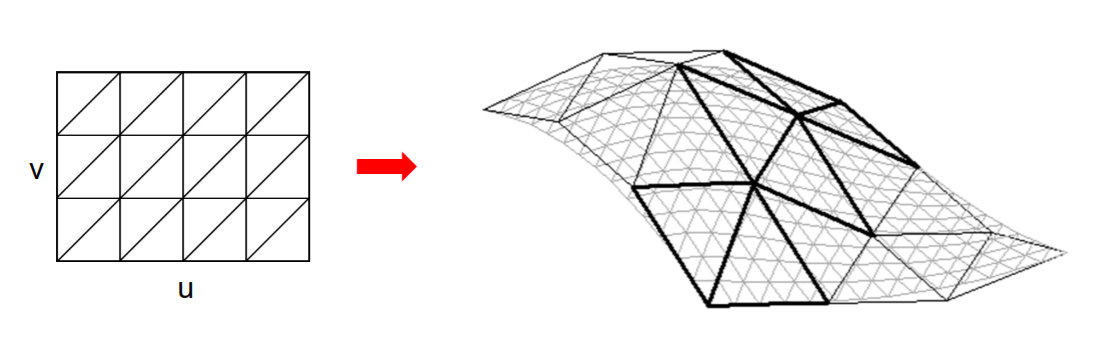
\includegraphics[height = 3.0cm]{ordinary_uv_to_mesh.png}
    \caption{triangulation in u,v parameter space}
\end{figure}
Just evaluate $(u, v)$ by uniform distribution, which may lost accuracy at some points (such as high curvature points or between very far neighbor control points).
\subsection{Adaption Mesh Construction}
My aim is to solve two problems:
\begin{itemize}
    \item [1)] high curvature points needs more vertex to render
    \item [2)] neighbor evaluated vertex may be too far between due to far neighbor control points.
\end{itemize}

\begin{figure}[h]
    \centering
    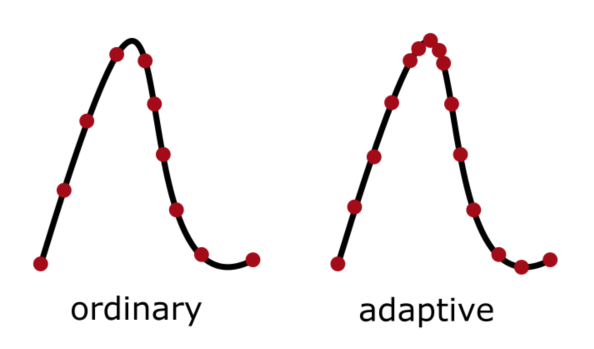
\includegraphics[height = 3.0cm]{ordinary_vs_adaptive.png}
    \caption{ordinary vs adaptive evaluation}
\end{figure}
So I imply a binary search adaptive mesh construction algorithm as follows:
\begin{lstlisting}[language=C++]
(u_v_list, vertex_list) adaptiveSub(low_v, high_v,
                      low_position, high_position):
    mid_v = (low_v + high_v)/2
    mid_position = evaluate(u, mid_v)
    mid_curvature = curvature(u, mid_v)
    resolution = distance(low_position, high_position)
    if (resolution >= curvature_distance_epsilon) and
       (mid_curvature >= curvature_max_rate) or
       (resolution >= distance_epsilon):
       temp_u_v_list += [(u, mid_v)]
       temp_vertex_list += [mid_position]
       temp_u_v_list, temp_vertex_list +=
       adaptiveSub(low_v, mid_v,
                   low_position, mid_position)
       temp_u_v_list, temp_vertex_list +=
       adaptiveSub(mid_v, high_v,
                   mid_position, high_position)
    return (temp_u_v_list, temp_vertex_list)
\end{lstlisting}
And we can do the same on both $u, v$,then we get a $(u,v)$ list and a vertex list.
After triangulate the $(u,v)$ map by Delaunator Algorithm, project the $(u,v)$ map to the 3D area.
Finally we can get a smooth enough adaptive Bézier Surface. And my algorithm's efficient is about 4 times slower then the ordinary one.

\subsection{B-Spline}
B-spline is defined by n order basis B-spline which can be derived by means of the Cox–de Boor recursion formula.
$$
    B_{i,0}(x):=\left\{{\begin{matrix}1&\mathrm {if} \quad t_{i}\leq x<t_{i+1}\\0&\mathrm {otherwise} \end{matrix}}\right.
$$
$$
    B_{i,k}(x):={\frac {x-t_{i}}{t_{i+k}-t_{i}}}B_{i,k-1}(x)+{\frac {t_{i+k+1}-x}{t_{i+k+1}-t_{i+1}}}B_{i+1,k-1}(x)
$$
So we can get BasisFunctions as follows:
\begin{lstlisting}[language=C++]
vector<float> basisFunctions(int i, float t) {
    vector<float> coeff, left, right;
    coeff.resize(degree + 1);
    left.resize(degree + 1);
    right.resize(degree + 1);
    coeff[0] = 1.0;

    for (auto j = 1; j <= degree; ++j) {
        left[j] = t - knot_vector[i + 1 - j];
        right[j] = knot_vector[i + j] - t;
        float saved = 0.0;
        for (auto r = 0; r < j; r++) {
            float tmp = coeff[r] /
                        (right[r + 1] + left[j - r]);
            coeff[r] = saved + tmp * right[r + 1];
            saved = tmp * left[j - r];
        }
        coeff[j] = saved;
    }
    return coeff;
}
\end{lstlisting}
Then we can evaluate every vertex and draw the surface.

\section{Results}
\subsection{Single Bézier Surface: Ordinary and Adaptive}
\begin{figure}[h]
    \centering
    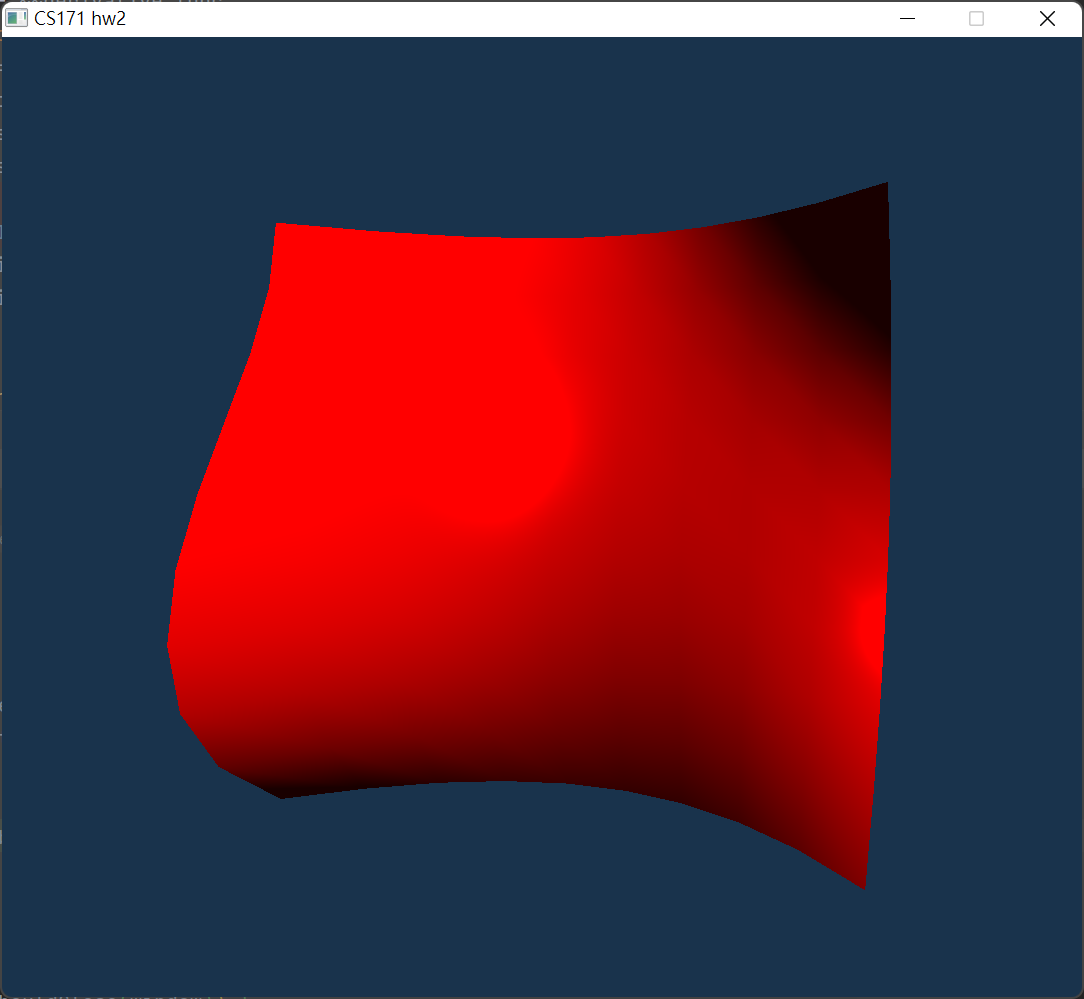
\includegraphics[height = 4.0cm]{ordinary_object.png}
    \caption{ordinary evaluation}
\end{figure}
\begin{figure}[h]
    \centering
    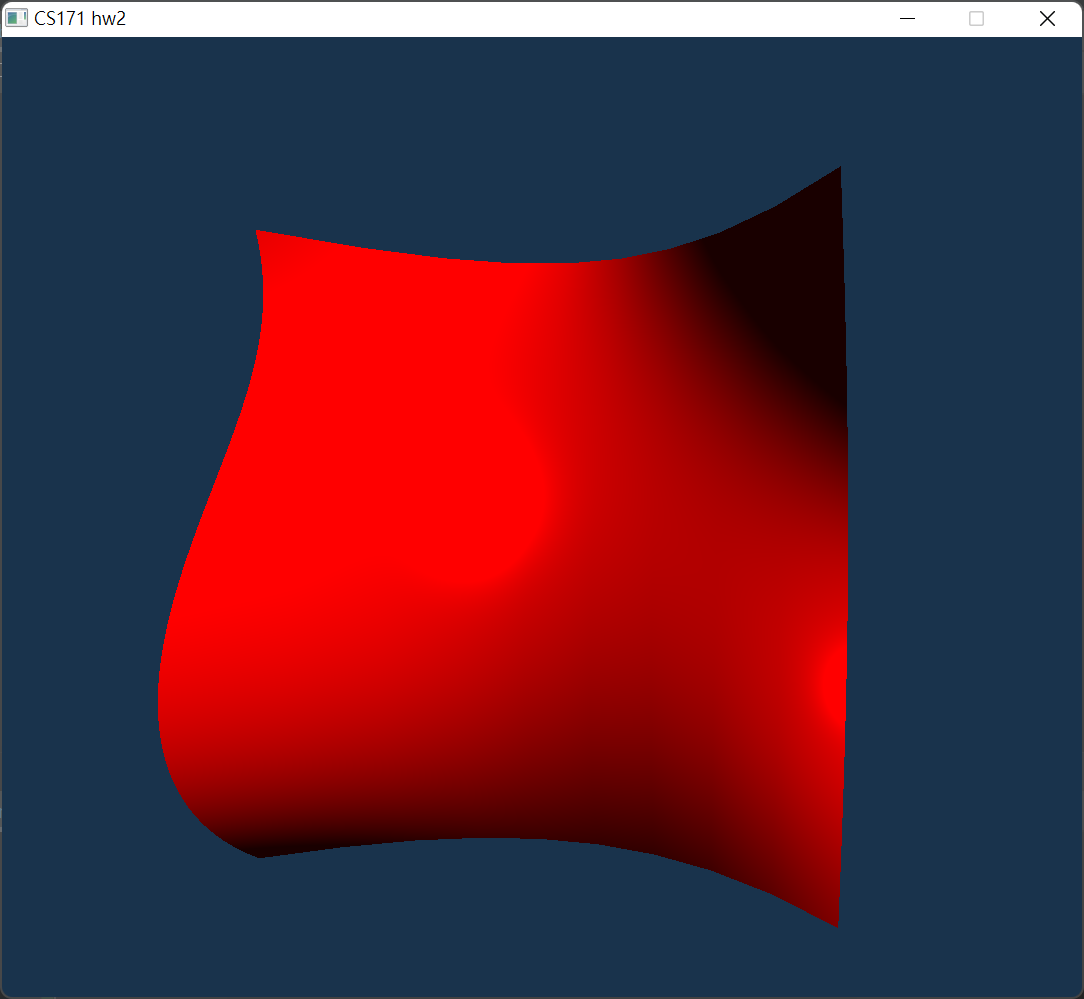
\includegraphics[height = 4.0cm]{adaptive_object.png}
    \caption{adaptive evaluation}
\end{figure}
\subsection{Complex Object: Teapot, Teacup and Teaspoon}
\begin{figure}[h]
    \centering
    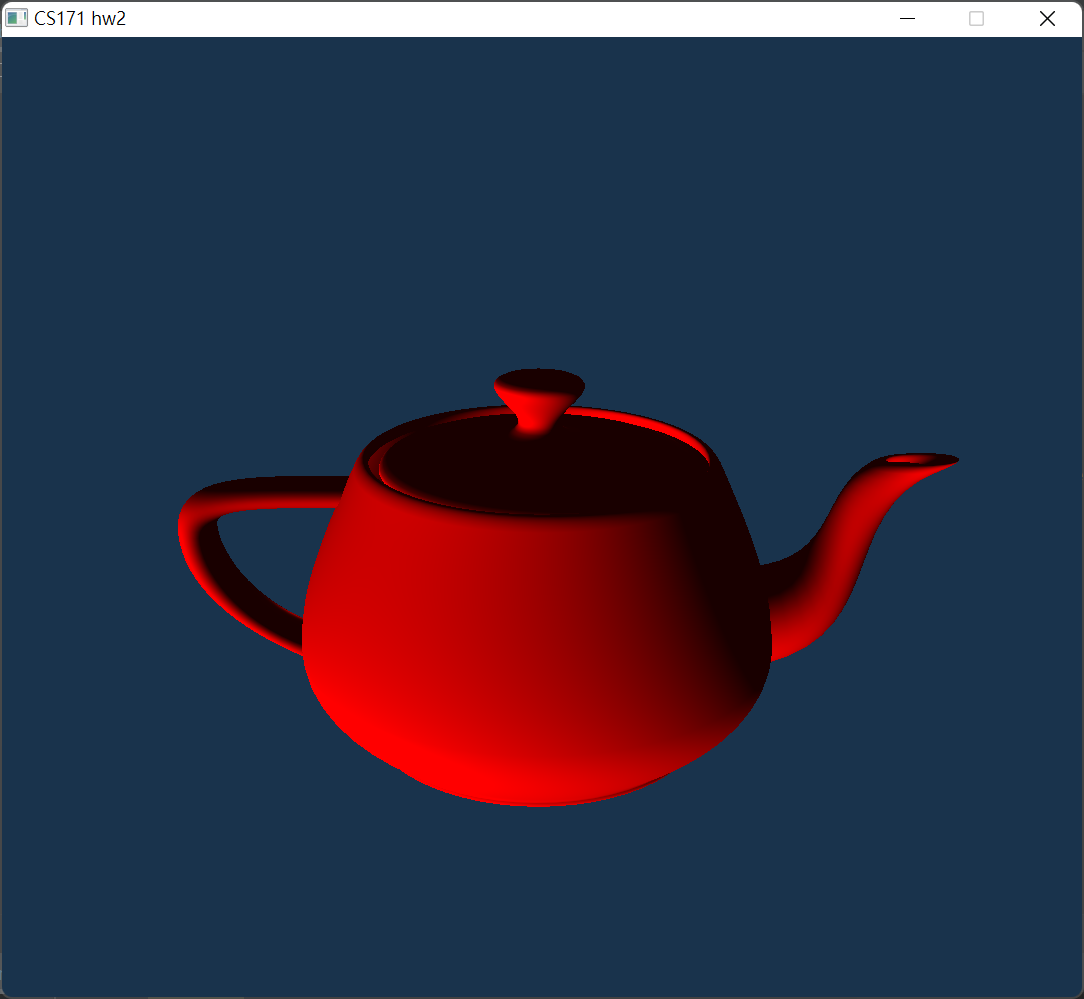
\includegraphics[height = 4.0cm]{teapot_all.png}
    \caption{Utah Teapot}
\end{figure}
\begin{figure}[h]
    \centering
    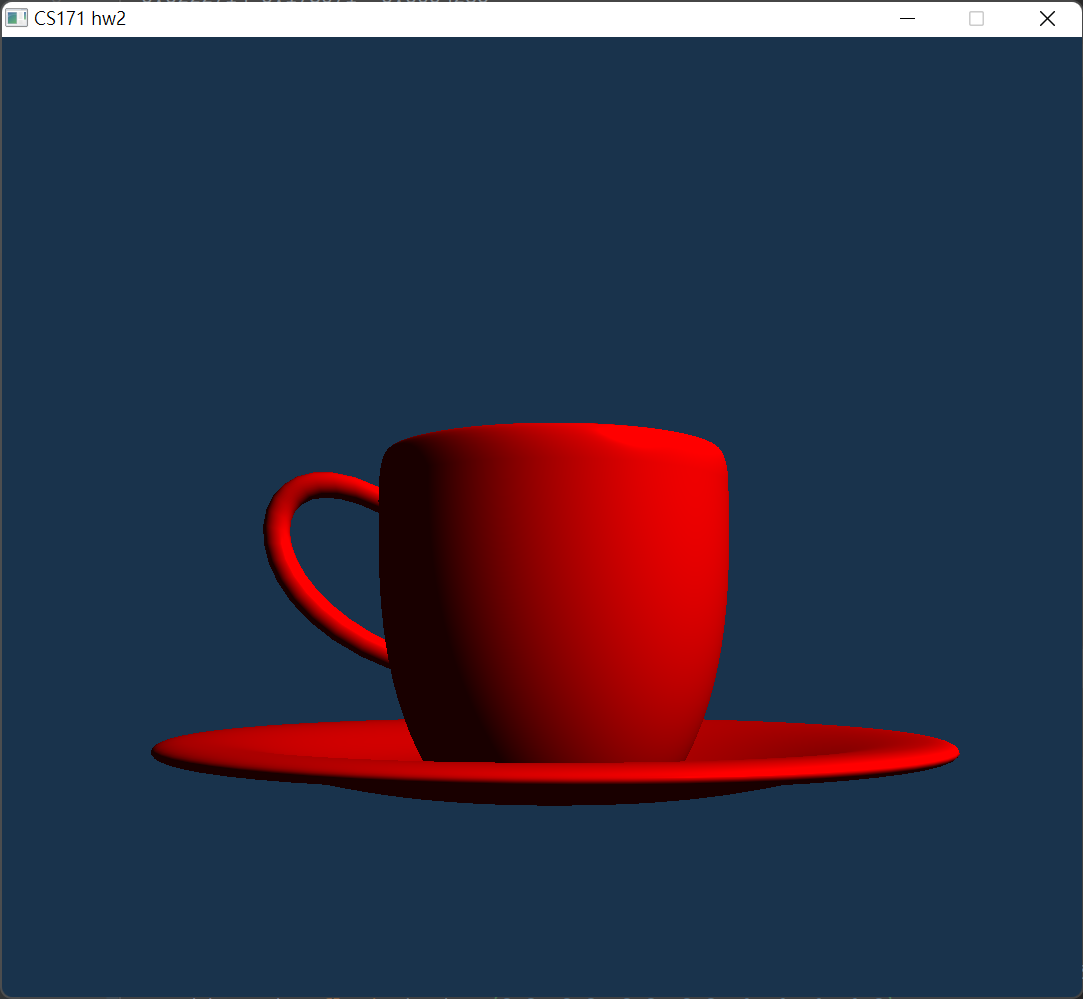
\includegraphics[height = 4.0cm]{teacup.png}
    \caption{Teacup}
\end{figure}
\begin{figure}[h]
    \centering
    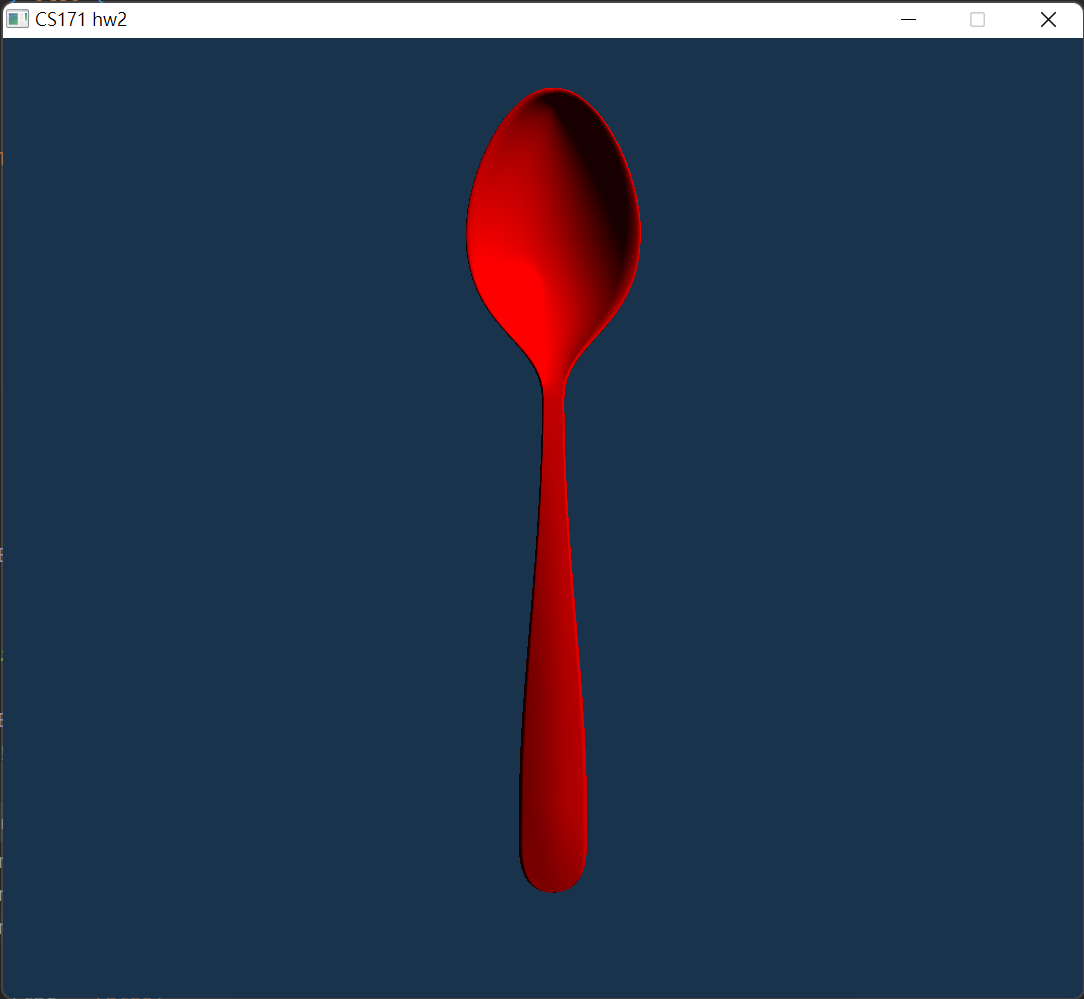
\includegraphics[height =4.0cm]{teaspoon.png}
    \caption{Teaspoon}
\end{figure}
\\
\subsection{B-Spline}
\\
\begin{figure}[H]
    \centering
    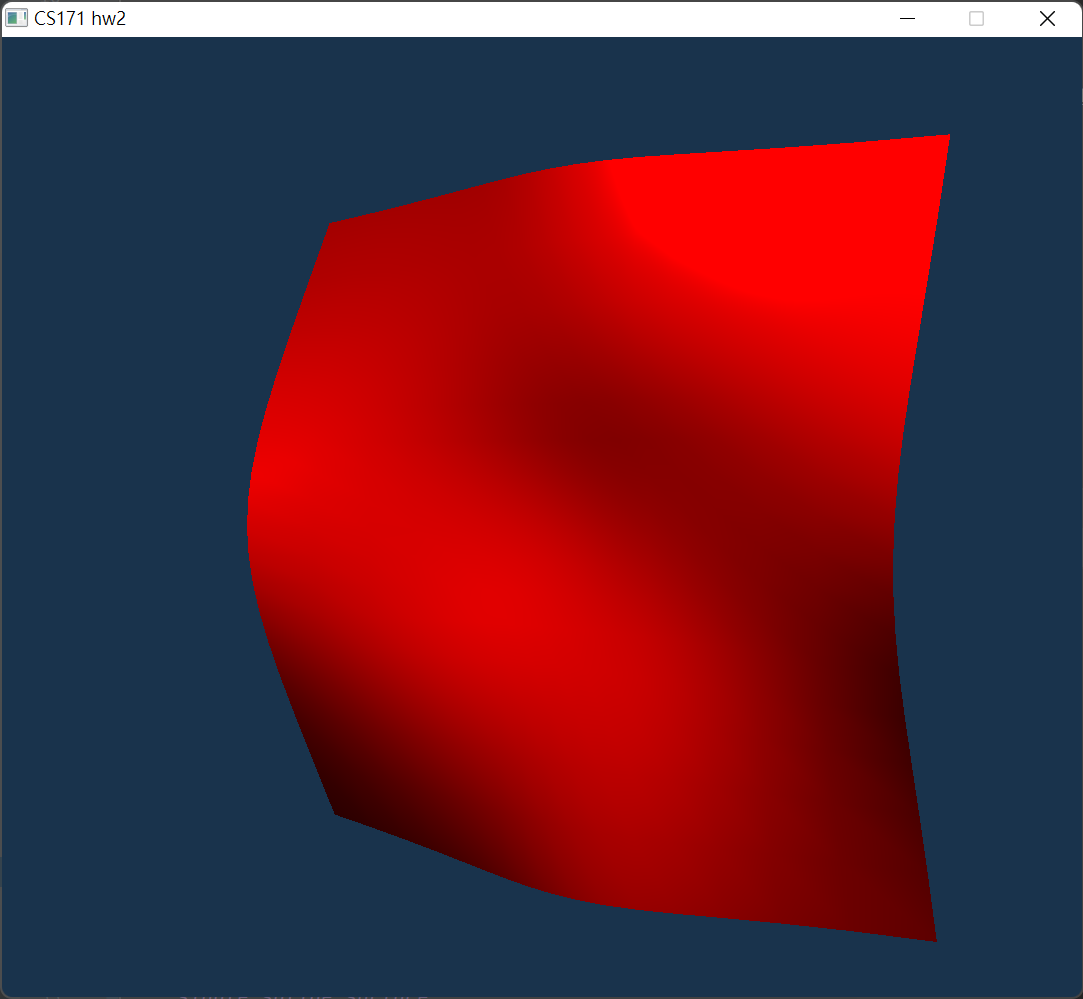
\includegraphics[height = 4.0cm]{bspline_surface.png}
    \caption{B-Spline Surface}
\end{figure}
\end{document}